\section{A Budget--Stakes Law: What a Sublinear Test Can and Cannot
Buy}

Every experiment above met the same wall: on average-case matching the
advice-free baseline is near-optimal, so predictions buy robustness
insurance rather than performance, and --- for the test-and-fallback
algorithms --- no acceptance threshold both captures the (tiny) upside
and stays safe (§5.3). This section quantifies the wall. The result is a
two-sided \textbf{budget--stakes law}: on a natural instance family,
deciding whether to follow the advice requires a prefix of length
\(k^* = \tilde\Theta(\sigma^2/g^2)\) --- the instance's specialist mass
(exactly twice its baseline slack) divided by the square of the stakes
\(g\) --- with \textbf{no} decision rule whatsoever simultaneously
consistent and robust below the budget (Theorem 1(i)) and an explicit,
embarrassingly simple rule succeeding at it (Theorem 1(ii)). The two
sides meet, up to logarithms, whenever the stakes are carried at
comparable signal levels by a constant fraction of the specialist mass
--- the condition under which ``\(k^*\)'' names one quantity rather than
two; when instead the stakes hide in a vanishing sliver of low-signal
cells the sides can separate, and we leave that regime open (§7.8). The
corollary is the wall: stakes are capped by the baseline slack, so on
strong-baseline instances meeting that condition the required prefix
exceeds the entire horizon --- any upside smaller than
\(\approx 2\sqrt{(1-\rho_{\mathrm{base}})/n}\) is uncapturable at
\emph{every} \(k\le n\), and the upsides we measured in §3--§5 sit in
exactly that range.

En route we record an honest negative of independent interest (§7.7):
the natural conjecture --- that the \(\tilde\Theta(r/\log r)\) hardness
of \emph{tolerant distribution testing}
\cite{canonne2022tolerance,valiant2011unseen,jiao2018l1} makes the
follow/fallback decision itself hard for any rule at sublinear \(k\) ---
is \textbf{false}. The advice's \emph{distance} \(\ell_1(p,q)\) is
indeed hard to test, and the empirical-\(\ell_1\) rules the field
actually uses \cite{choo2024imperfect,bem2026testmatch} are provably
blind at \(k \ll r\); but the decision-relevant functional is the
\emph{payoff} of following, which on decomposable instances collapses to
a per-sample observable. Testing the payoff is exponentially cheaper
than testing the prediction.

\textbf{Relation to prior work.} Choo et al.~\cite{choo2024imperfect}
and Burathep--Erlebach--Moses \cite{bem2026testmatch} give \emph{upper}
bounds (algorithms) in this model and no statistical lower bound; Choo
et al.'s Thm 3.1 is the generic adversarial trade-off (no algorithm is
\(1\)-consistent and \(>\tfrac12\)-robust), driven by adversarial
instances, not by the resolution of a sublinear test. Their acceptance
threshold \(\tau = 2(\hat n/n-\beta)-\varepsilon\) couples to the
baseline \(\beta\) \emph{constructively}; Theorem 1(i) is the
information-theoretic counterpart --- it binds \emph{every} measurable
rule on the prefix. The consistency/robustness lower bounds elsewhere in
the with-predictions literature \cite{weizhang2020tradeoffs} are
problem-intrinsic Pareto frontiers, not gated by a test.
Tolerant-testing sample complexity \cite{canonne2022tolerance} enters
our story twice, both times off the critical path: it explains
\emph{why} the field's \(\ell_1\)-threshold rules are blind (§7.7), and
its hard instances are exactly what our payoff identity (Lemma 2)
sidesteps. To our knowledge, both the budget--stakes law and the
observation that payoff-testing strictly separates from distance-testing
in an online algorithm are new. A dedicated pass over the adjacent lines
(§9) found none testing the payoff: the \emph{test-before-trust} program
of Choo, Gouleakis and coauthors
\cite{choo2024imperfect,bhattacharyya2025product} validates advice by
distributional distance throughout --- exactly the statistic §7.7 shows
is the wrong one on average-case inputs; switching frameworks
\cite{chledowski2021caching,antoniadis2025switching} switch dynamically
on prediction quality or regret rather than committing on a payoff test,
and matching's irrevocability breaks them (§5.5); data-driven algorithm
selection \cite{gupta2017pac,balcan2020datadriven} chooses among
algorithms from samples of \emph{whole instances} with observable
per-instance performance, and best-arm identification prices the same
two-way choice at \(\Theta(1/g^2)\) \emph{active pulls} whose rewards
are directly observed \cite{mannortsitsiklis2004,kaufmann2016complexity}
--- whereas here a single instance's prefix is a passive arrival stream,
containing neither actions nor rewards, and it must nonetheless reveal a
policy pair's full-horizon value gap --- which is precisely what the
payoff identity provides and what the lower half shows no rule can
extract faster; and the \(1/g^2\) budget itself echoes classical
sequential analysis \cite{wald1947sequential}, whose engine --- not its
novelty --- Lemma 2 imports into matching.

\subsection{The test-and-fallback
class}

Fix an instance family and a budget \(k=o(n)\). A
\textbf{test-and-fallback} algorithm \(A_k\) observes the first \(k\)
arrivals \(X_{1:k}\) and the advice \(\sigma\), outputs a (possibly
randomized) decision \(D\in\{\mathsf{Follow},\mathsf{Fallback}\}\) as a
function of \((X_{1:k},\sigma)\), and thereafter Mimics \(\sigma\) if
\(D=\mathsf{Follow}\) and runs the advice-free baseline \(B\) (Ranking)
otherwise. Because \(k=o(n)\), the prefix's own contribution to the
ratio is \(O(k/n)=o(1)\), absorbed below. Write \(\rho_{\mathrm{base}} =
\mathbb E[B]/\mathrm{OPT}\) for the baseline strength,
\textbf{consistency} for the ratio under good advice, and
\textbf{robustness} for the ratio under adversarial advice.

\subsection{The master trade-off
(rigorous)}

\begin{quote}
\textbf{Lemma 1.} Let \(G,\mathrm{Bd}\) be two instance distributions
sharing the \emph{same} advice \(\sigma\), with prefix laws
\(\mathcal L_G,\mathcal L_{\mathrm{Bd}}\) and
\(\gamma_k:=\mathrm{TV}(\mathcal L_G,\mathcal L_{\mathrm{Bd}})\).
Suppose following \(\sigma\) gains \(\delta\) under \(G\) and loses
\(\Delta\) under \(\mathrm{Bd}\) relative to \(B\). Parameterize \(A_k\)
by the fraction \(\eta_c\) of the upside it forgoes under \(G\) and its
robustness loss \(\eta_r\Delta\) under \(\mathrm{Bd}\). Then
\[(1-\eta_c)\;\le\;\eta_r+\gamma_k+o(1).\]
\end{quote}

\emph{Proof.} Conditioning on \(D\) under \(G\),
\(\mathbb E_G[A_k]/\mathrm{OPT} = P_G(\mathsf F)\,
\mathbb E_G[\mathrm{Mimic}]/\mathrm{OPT} + P_G(\mathsf R)\rho_{\mathrm{base}} \pm o(1) \ge
\rho_{\mathrm{base}} + \delta\,P_G(\mathsf F)-o(1)\), so the captured
upside \((1-\eta_c)\delta\) forces \(P_G(\mathsf F)\ge 1-\eta_c-o(1)\).
Symmetrically \(P_{\mathrm{Bd}}(\mathsf F)=\eta_r
+o(1)\). Since \(D\) is a function of \((X_{1:k},\sigma)\) and
\(\sigma\) is identical,
\(|P_G(\mathsf F)-P_{\mathrm{Bd}}(\mathsf F)|\le\gamma_k\); chaining
gives the claim. \(\qed\)

In the form that sets the prefix's own \(O(k/n)\) aside by defining
values as post-decision ratios, the inequality is exact ---
\((1-\eta_c)\le\eta_r+\gamma_k\) with no \(o(1)\) --- for every finite
prefix space and every \([0,1]\)-valued rule; that is the form
machine-checked in Appendix C (\texttt{Scenario.master\_tradeoff}).

With an \emph{uninformative} prefix (\(\gamma_k=o(1)\)) one cannot be
both near-fully-consistent (\(\eta_c\to0\)) and robust (\(\eta_r\to0\)).
Everything below is a computation of how large \(k\) must be before the
prefix becomes informative --- and (the half the earlier draft missed)
of how \emph{small} a \(k\) already suffices.

\subsection{The construction and the affine
law}

The family is a disjoint union of \(m\) independent
\textbf{rare-resource cells}, each over a distinct type-pair, so the
support is \(r=\Theta(m)\) and (at \(m = \Theta(n)\)) each type is seen
\(O(1)\) times. Cell \(i\) has resources \(\{a_i,b_i\}\), a flexible
request (neighborhood \(\{a_i,b_i\}\)) that must be routed before a
specialist (\(\{a_i\}\) or \(\{b_i\}\), present with probability
\(\theta_i\)) is seen; the right route depends on the future specialist.
The profile \(\{(\theta_i,\varepsilon_i)\}_{i\le m}\) is
\textbf{arbitrary} --- no homogeneity is assumed anywhere below. In
closed form (verified numerically), cell \(i\) has
\(\mathrm{OPT}=1+\theta_i\), baseline \(1+\theta_i/2\), and following
the advice gains or loses exactly \(\theta_i\lvert s_i-\tfrac12\rvert\)
over the baseline according to whether the advice's \emph{direction} is
right, where \(s_i = \tfrac12 \pm \varepsilon_i\) is the specialist bias
and \(\varepsilon_i\) the signal; the advice-to-truth distance is
\(\ell_1=2\theta_i\lvert s_i-\hat s_i\rvert\) per cell.

These aggregate cleanly. Summing over cells yields an \textbf{exact
affine law} (proven, and machine-checked from the cell constants,
Appendix C; verified to three decimals):
\[\mathbb E[\text{follow-ratio}] \;=\; \rho_{\mathrm{perfect}} - \tfrac12\,\ell_1(p,q),
\qquad \ell_1^\star \;=\; 2\big(\rho_{\mathrm{perfect}}-\rho_{\mathrm{base}}\big),\]
where \(\rho_{\mathrm{perfect}}\) is the all-correct-direction ratio and
\(\ell_1^\star\) the break-even. The quantity that organizes everything
is the family's \textbf{specialist mass}
\[\sigma^2 \;:=\; \frac{\sum_i \theta_i}{N}, \qquad N=\sum_i(1+\theta_i)=\mathrm{OPT}\]
--- the probability that a random arrival is a specialist, and (below)
the variance bound on the decision statistic. Two exact identities (both
machine-checked, Appendix C) anchor what follows: the baseline slack
\emph{is} half the specialist mass,
\[1-\rho_{\mathrm{base}} \;=\; \sigma^2/2,\] and the maximum stakes (the
full upside) are
\(\rho_{\mathrm{perfect}}-\rho_{\mathrm{base}} = \sum_i\theta_i\varepsilon_i/N
\le 2\varepsilon_{\max}\,(1-\rho_{\mathrm{base}})\): \emph{the upside is
at most an \(\varepsilon\)-fraction of the baseline slack.} That the
same \(\sigma^2\) measures both the slack and the noise is not a
coincidence --- it is the law. The canonical (verified) instantiation
takes \(\theta_i=\theta\), \(\varepsilon_i=\varepsilon\) and a
wrong-direction fraction \(\varphi=\tfrac14\) (good: \(\ell_1 = a\),
gain \(\delta\)) versus \(\varphi=\tfrac34\) (bad: \(\ell_1 = b\), loss
\(\Delta\)), with \(\delta=\Delta=\ell_1^\star/4\).

\subsection{The payoff identity: the stakes are a per-sample
observable}

The earlier route tried to make the follow/fallback decision \emph{hard}
by making \(\ell_1(p,q)\) hard to test. On this family that cannot work,
for a reason worth a lemma. Classify each arrival by its role in its own
cell, relative to the advice's predicted direction:
\[c(X) \;=\; \begin{cases} +1 & X \text{ is the advice-favored specialist of its cell,} \\
-1 & X \text{ is the disfavored specialist,} \\ 0 & X \text{ is flexible.}\end{cases}\]

\begin{quote}
\textbf{Lemma 2 (payoff identity).} For every type distribution \(p\) on
the family --- any profile \(\{(\theta_i,\varepsilon_i)\}\), and any
truth biases \(s_i\in[0,1]\), matching the advice's magnitudes or not
---
\[\mathbb E_p[c] \;=\; \frac2N\sum_i \theta_i\,(s_i-\tfrac12)\,\hat d_i
\;=\; 2\cdot\frac{\mathbb E_p[\mathrm{Mimic}]-\mathbb E_p[B]}{\mathrm{OPT}}.\]
\emph{The expected advantage of following the advice is half the mean of
a bounded, per-sample observable.} (Machine-checked from the cell
constants --- \texttt{CellFamily.payoff\_identity}, Appendix C; verified
to three decimals by \texttt{verify\_witness\_gap.py} for homogeneous
wrong-fraction sweeps, and by \texttt{verify\_budget\_stakes\_hetero.py}
for random heterogeneous and magnitude-mismatched profiles.)
\end{quote}

\emph{Proof.} The advice-favored and disfavored specialists of cell
\(i\) have masses \(\theta_i\,(\tfrac12\pm(s_i-\tfrac12)\hat d_i)/N\),
where \(\hat d_i\) is the advice direction; so cell \(i\) contributes
\(2\theta_i(s_i-\tfrac12)\hat d_i/N\) to \(\mathbb E[c]\), while by the
cell constants its follow-advantage is
\(\theta_i(s_i-\tfrac12)\hat d_i\). Sum over cells and divide by
\(\mathrm{OPT}=N\). \(\qed\)

\subsection{The budget--stakes law}

\textbf{Symbols.} One quantity carries the stakes and one pair carries
its two directions. For a scenario pair \((G,\mathrm{Bd})\) sharing an
advice, \(g\) is the \textbf{payoff gap} --- the difference in
follow-advantage between the two scenarios --- while \(\delta\) and
\(\Delta\) are the gain under \(G\) and the loss under \(\mathrm{Bd}\)
separately, the objects Lemma 1 is stated in. By definition
\(g=\delta+\Delta\), so \(\min(\delta,\Delta)\le g/2\) always, with
equality exactly when the pair is \textbf{balanced}. The flip pairs of
(i) are balanced --- flipping the cells of \(W\) moves each \(s_i\)
symmetrically about \(\tfrac12\), giving \(\delta=\Delta=g/2\) --- so on
them \(\min(\delta,\Delta)=\Theta(g)\) and the two halves below
constrain the same quantity. On an unbalanced pair (ii) is governed by
the smaller of the two directions, and it is \(\min(\delta,\Delta)\),
not \(g\), that sets the budget.

\begin{quote}
\textbf{Theorem 1 (budget--stakes law, heterogeneous).} On any cell
family with profile \(\{(\theta_i,\varepsilon_i)\}\) and specialist mass
\(\sigma^2\):

\textbf{(i) (Impossibility below the budget --- any rule.)} Let
\(G,\mathrm{Bd}\) be the scenario pair that flips the advice-agreement
of a cell set \(W\) whose signals are at most \(\varepsilon_W\), with
payoff gap \(g=\tfrac2N\sum_{i\in W}\theta_i\varepsilon_i\). Every
test-and-fallback algorithm \(A_k\), deciding by \emph{any} measurable
rule on the prefix, with \(k \,=\, o\!\big(1/(\varepsilon_W\,g)\big)\)
has \(\eta_c+\eta_r \ge 1-o(1)\): it forgoes the upside or eats the
loss.

\textbf{(ii) (The budget suffices --- an explicit rule.)} For \emph{any}
pair of truth profiles --- magnitudes need not match the advice --- on
which following gains \(\ge\delta\) and loses \(\ge\Delta\), the
\textbf{directional test} --- follow iff \(\sum_{j\le k} c(X_j) > 0\)
--- achieves \(\eta_c+\eta_r \le \epsilon_0\) once
\(k \ge C\,(\sigma^2/\min(\delta,\Delta)^2)\log(1/\epsilon_0)\). In
particular \(k\) is \emph{independent of \(n\)} for constant stakes.

The two sides meet up to logarithms whenever the stakes are carried, at
comparable signal levels, by a constant fraction of the specialist mass
(Cauchy--Schwarz:
\(g^2 \le \tfrac4N\sigma^2_W\sum_W\theta_i\varepsilon_i^2\),
\(\sigma^2_W\) the flipped mass) --- in particular for the canonical
pair, giving the critical budget
\[k^* \;=\; \tilde\Theta\!\big(\sigma^2/g^2\big),\] which at homogeneous
parameters is the earlier \(\tilde\Theta(\theta/\delta^2)\).
\end{quote}

\emph{Proof of (ii).} By Lemma 2, \(\mathbb E[c] \ge 2\delta\) under the
gain scenario and \(\le -2\Delta\) under the loss scenario, for any
truth profile;
\(\mathrm{Var}(c) \le \mathbb P(\text{specialist}) = \sigma^2\);
Bernstein's inequality gives error
\(\exp(-\Omega(k\min(\delta,\Delta)^2/\sigma^2))\) on both sides.
\(\qed\) (Explicit constants, machine-checked in Appendix C:
\texttt{iid\_prob\_sum\_nonpos\_le} gives, without the variance
refinement, error at most \(e^{-k\min(\delta,\Delta)^2}\);
\texttt{iid\_prob\_sum\_nonpos\_le\_cheb} gives the \(\sigma^2\)-scaling
at Chebyshev grade, error at most
\(\sigma^2/(4k\min(\delta,\Delta)^2)\); Bernstein's exponential
\(\sigma^2\)-dependence is the one step of the upper half taken from the
textbook rather than the kernel.)

\emph{Proof of (i), in outline (in full in Appendix B).} Couple the two
scenarios; the per-sample laws differ only on the specialists of the
flipped cells, and the per-sample squared Hellinger distance is exactly
\(H^2 = \sum_{i\in W}\tfrac{2\theta_i}{N}\big(1-\sqrt{1-4\varepsilon_i^2}\big)
\in [4,8]\cdot\sum_{i\in W}\theta_i\varepsilon_i^2/N \le 4\,\varepsilon_W\,g\).
Tensorizing the Bhattacharyya coefficient and passing to total variation
gives \(\gamma_k \le \sqrt{k\,H^2} = o(1)\) whenever
\(k = o(1/(\varepsilon_W g))\), and Lemma 1 turns that into
\(\eta_c+\eta_r\ge 1-o(1)\) (these last steps, chained with Lemma 1, are
machine-checked: \texttt{Scenario.master\_tradeoff\_iid}, Appendix C).
\(\qed\)

Numerically (§\texttt{verify\_witness\_gap.py}, \(\theta=0.6\),
\(\varepsilon=0.3\), \(\delta=0.056\)): the directional test reaches
\(\eta_c+\eta_r \approx 0.06\) at \(k=100\) and \(0.007\) at \(k=200\),
and stays flat as \(n\) grows from \(3{,}200\) to \(320{,}000\) at fixed
\(k=200\) --- the budget really is \(n\)-free once the stakes are
constant. The heterogeneous claims are verified separately
(\texttt{verify\_budget\_stakes\_hetero.py}): the payoff identity holds
for random profiles and for magnitude-mismatched truths;
\(1-\rho_{\mathrm{base}}=
\sigma^2/2\) exactly; the per-sample Hellinger distance sits inside its
\([4,8]\) bounds; and three families with
\(\sigma^2\in\{0.13,0.24,0.42\}\) produce decision-error curves that
\emph{coincide} as a function of \(k g^2/\sigma^2\) alone
(\(0.30/0.15/0.02/0.001\) at \(kg^2/\sigma^2=\tfrac14/1/4/8\)) --- the
budget--stakes scaling is the whole story. Section 5.4 carries the rule
from the hard family to the benchmark itself, where the plug-in payoff
must additionally survive a concavity bias at the capacity kinks --- it
does, with a bootstrap calibration that still uses no problem constants.

\subsection{The wall, quantified: strong baselines price the test out of
the
horizon}

Stakes are capped by the slack:
\(g \le \rho_{\mathrm{perfect}}-\rho_{\mathrm{base}}
\le 2\varepsilon_{\max}(1-\rho_{\mathrm{base}}) = \varepsilon_{\max}\,\sigma^2\).
Theorem 1 places the feasibility frontier at
\(g \asymp \sigma/\sqrt k\): a prefix of length \(k\) resolves stakes
down to \(\sigma/\sqrt k\) and no further. With the whole instance as
prefix (\(k=n\)), the constant-free threshold is
\[g^{*} \;=\; \sigma/\sqrt n \;=\; \sqrt{2(1-\rho_{\mathrm{base}})/n}\,:\]

\begin{quote}
\textbf{Corollary (uncapturable upsides).} On strong-baseline families
satisfying the matching condition of Theorem 1 --- the stakes carried at
comparable signal levels by a constant fraction of the specialist mass
--- every advice upside smaller than
\(\Theta\big(\sqrt{(1-\rho_{\mathrm{base}})/n}\,\big)\) is uncapturable
by any test-and-fallback rule at any prefix length \(k \le n\) --- the
information needed to decide does not exist inside the instance.
(Theorem 1(ii) --- stakes above the frontier \emph{are} resolvable ---
is unconditional; it is the impossibility direction, and hence this
corollary, that inherits the condition.)
\end{quote}

At the parameters of our benchmark (§3:
\(\rho_{\mathrm{base}}\approx0.99\), \(n=2000\)) the threshold is
\(g^{*}\approx 0.003\), and the measured upsides are \(<0.01\) (F3) ---
the empirical wall sits in the regime the corollary governs. This is the
\textbf{scissors} of \textbf{Figure 8}
(\texttt{results/impossibility\_frontier.png}), now with the correct
mechanism: the \emph{potential} upside (perfect advice minus baseline)
grows as the baseline weakens, while the upside a feasible test can
safely capture is pinned by the \(\sqrt{(1-\rho_{\mathrm{base}})/n}\)
resolution --- \textbf{the structure that makes the baseline strong is
the structure that starves the test of signal.}

\begin{figure}
\centering
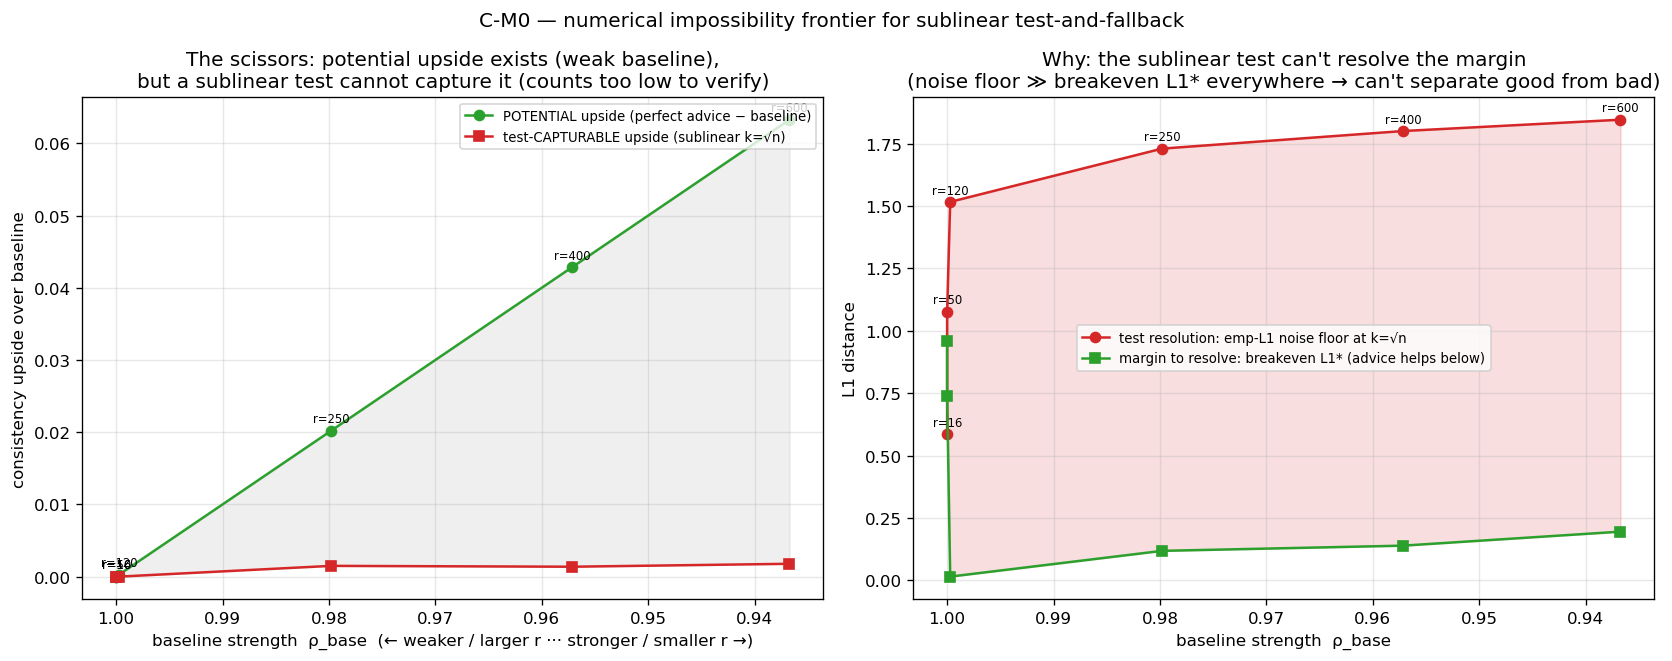
\includegraphics[width=1\linewidth,height=\textheight,keepaspectratio,alt={The budget--stakes scissors: as the baseline weakens (left), the potential upside of perfect advice grows, while the upside a feasible test can safely capture stays pinned near zero --- the empirical test's resolution sits far above the break-even margin wherever the upside exists.}]{../../results/impossibility_frontier.png}
\caption{The budget--stakes scissors: as the baseline weakens (left),
the potential upside of perfect advice grows, while the upside a
feasible test can safely capture stays pinned near zero --- the
empirical test's resolution sits far above the break-even margin
wherever the upside exists.}
\end{figure}

\subsection{Why the field's rules hit the wall earlier: distance-testing
is the wrong
statistic}

The algorithms of \cite{choo2024imperfect,bem2026testmatch} do not run
the directional test; they threshold the plug-in distance
\(\hat\ell_1(\hat p_k, q)\). That class is blind far before Theorem 1(i)
bites: at \(k \ll r\) the empirical \(\hat p_k\) is \(k\) atoms of mass
\(1/k\), so \(\hat\ell_1 \approx 2\) \emph{regardless of the advice's
quality} (numerically: \(1.908\) vs \(1.913\) on the two canonical
scenarios whose true \(\ell_1\) differ by \(0.225\)). Any threshold
therefore either always accepts or always rejects --- the §5.3
pathology, now explained. The same blindness is measurable on the
benchmark generator itself: holding the true error at
\(\ell_1\approx0.11\) and growing the support from \(r=8\) to \(512\) at
fixed \(k=200\), the plug-in estimate inflates from \(0.17\) to \(1.22\)
--- twelve times the truth --- while the payoff rule of §5.4 keeps
deciding, staying within the prefix cost of the floor at both good and
bad advice (\textbf{Figure 9}).

\begin{figure}
\centering
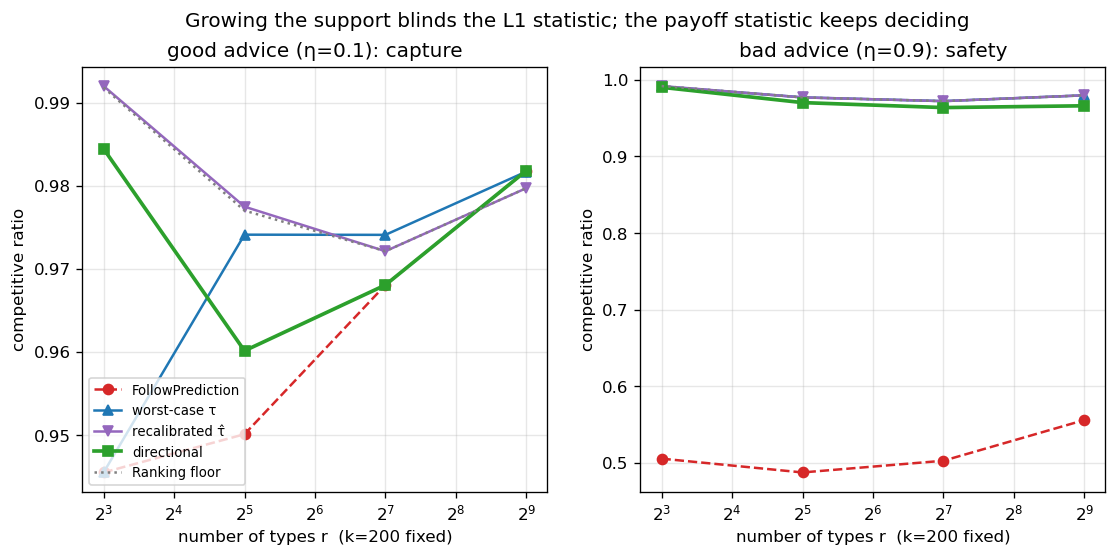
\includegraphics[width=1\linewidth,height=\textheight,keepaspectratio,alt={The blindness curve on the benchmark generator: at fixed true \textbackslash ell\_1\textbackslash approx0.11 and k=200, the plug-in \textbackslash hat\textbackslash ell\_1 inflates with the support size while the payoff rule keeps deciding at both good (left) and bad (right) advice.}]{../../results/directional_rsweep.png}
\caption{The blindness curve on the benchmark generator: at fixed true
\(\ell_1\approx0.11\) and \(k=200\), the plug-in \(\hat\ell_1\) inflates
with the support size while the payoff rule keeps deciding at both good
(left) and bad (right) advice.}
\end{figure}

The deeper reason is the tolerant-testing barrier: estimating
\(\ell_1(p,q)\) to constant accuracy at \(r=\Theta(n)\) genuinely
requires \(\tilde\Theta(n/\log n)\) samples \cite{canonne2022tolerance}.
The resolution of the apparent paradox --- the \emph{decision} is easy
(Theorem 1(ii)) while the \emph{distance} is hard --- is Lemma 2: the
payoff is a linear, per-sample functional, and \(\ell_1\) is not. The
practical moral for algorithm designers is one sentence: \textbf{test
the payoff, not the prediction.}

We record the flip side honestly. The natural conjecture behind an
earlier version of this section --- that tolerant-testing hardness makes
the follow/fallback decision itself impossible for \emph{any} rule at
\(k = o(n/\log n)\) with \(\Theta(1)\) stakes --- is \textbf{refuted} by
Theorem 1(ii): no witness pair with \(\gamma_k = o(1)\) and
\(\Theta(1)\) stakes exists on this family, because by Lemma 2 a
\(\Theta(1)\) stake gap forces \(\gamma_k \to 1\) at any
\(k=\omega(1)\). The tolerant-testing hard instances evade Lemma 2 only
by mismatching the advice's per-cell magnitudes --- precisely the regime
in which distance and payoff decouple and \(\ell_1\) stops being the
decision-relevant quantity.

\subsection{Scope and honesty}

Both halves of Theorem 1 use only elementary tools (Bernstein; Hellinger
tensorization plus Lemma 1) --- deliberately: the earlier,
stronger-sounding route through tolerant-testing lower bounds is closed
by §7.7, and we consider the refutation itself part of the contribution.
The tools are elementary enough that the entire chain --- the three
identities of §7.3--7.4, Lemma 1 in exact form, and both halves of the
law at the abstract level (a finite Chernoff bound above, Hellinger
tensorization below) --- is formalized in Lean 4 over Mathlib and
accepted by its kernel: 66 theorems and lemmas, no \texttt{sorry},
shipped in the artifact (Appendix C). We offer the kernel certificate in
place of heavier machinery, and list there what the formalization does
\emph{not} cover --- the cell constants, the explicit Hellinger
evaluation on the family, and Bernstein's \(\sigma^2\)-dependent
exponent. The law now allows fully heterogeneous cell profiles, and its
achievability side holds for arbitrary (magnitude-mismatched) truth
distributions --- neither homogeneity nor the matched-magnitude advice
model is load-bearing. Its two sides can separate, by the factor
\(\sigma^2\varepsilon_W/g \ge 1\), when a scenario pair's stakes hide in
an asymptotically vanishing sliver of low-signal cells; closing that
regime is open. The law is stated for decomposable (disjoint-cell)
families; by Lemma 2 the payoff is per-sample observable on \emph{every}
such family, so no decomposable construction can restore a
super-\(1/\delta^2\) barrier. Whether a \emph{non-decomposable} family
--- long-range dependence making the payoff a genuinely hard functional
--- can separate the budget from \(1/\delta^2\) is open. The directional
test is analyzed here only on the cell family; a dedicated novelty pass
--- whose venues, keywords and cut-off are stated in §9 --- found no
payoff-testing acceptance rule in the adjacent literatures --- the
nearest lines test distances, switch on regret, or select algorithms
from whole-instance samples (§9) --- though the statistical skeleton of
the upper half is, deliberately, classical. We credit Choo et al.~for
the constructive baseline-coupling their threshold already exhibits; our
contribution is the two-sided, rule-independent budget law, the
payoff/distance separation, and the quantified wall.

\textbf{Remark (random order).} The law's scaling is not tied to i.i.d.
arrivals. In the random-order model --- a fixed population of \(n\)
arrivals presented in a uniformly random order, the algorithm deciding
on the first \(k\) --- both halves persist. \emph{Lower half:} an
adversary who draws the population i.i.d. from \(P\) (respectively
\(Q\)) and presents it in random order presents exactly the product law,
because a uniformly shuffled i.i.d. sample is i.i.d.
(\texttt{shuffled\_iid\_expect}, Appendix C); Theorem 1(i) therefore
binds every random-order rule as stated, up to the \(o(1)\) by which the
stakes of a random population concentrate at their mean. \emph{Upper
half:} on a fixed population the payoff identity holds pathwise (the
favored-minus-disfavored specialist count is twice the realized
follow-advantage, and \(\mathrm{OPT}=n\)), and the directional statistic
is a sum without replacement whose variance is at most
\(k\,\mathbb E_{\mathrm{pop}}[c^2]=k\sigma^2_{\mathrm{pop}}\) (the
finite-population correction only helps), so the directional test errs
with probability at most
\(\sigma^2_{\mathrm{pop}}/(4k\min(\delta,\Delta)^2)\)
(\texttt{ro\_prob\_sum\_nonpos\_le}, Appendix C) --- the same budget, at
Chebyshev grade; the exponential form follows from Hoeffding's
without-replacement theorem \cite{hoeffding1963probability} (or
Serfling's sharpening \cite{serfling1974probability}), which we cite
rather than reprove. What does \emph{not} transfer is the empirical wall
of §3--§6, which is an average-case statement.
